\section{Benchmark}

Pour évaluer notre implémentation nous avons réalisé un petit benchmark qui se charge de simuler un
scénario basique.

\noindent \textbf{Scénario:}
Nous voulons tester un scénario comparable à celui présenté dans la partie \textbf{4.1 Monocœur}.
Un thread parent prend un mutex et lance l'exécution de N threads enfant se bloquant sur son mutex.
Une fois les enfants lancés, le parent exécute son calcul.
X autres threads s'exécutent en parallèle du thread parent et effectue leur calcul.
Le programme s'arrête brutalement quand le parent a fini l'exécution de son calcul.

\noindent \textbf{Calcul des threads:} 
Calcul du déterminent d'une matrice 11x11.

\noindent \textbf{Résultat attendu:}
Les N threads enfant doivent augmenter la priorité du thread parent de N. Le thread parent doit donc voir son temps d'exécution significativement réduit en fonction de N et finir avant les X threads parallèles.

\noindent \textbf{Environnement de test:}
Machine virtuelle avec 1 cœur.


\begin{figure}[h!]
	\centering
	\begin{tikzpicture}
	\begin{axis}[
	xlabel={Nombre de threads N enfants},
	ylabel={Temps d'exécution du parent (s)},
	xmin=0, xmax=50,
	ymin=0, ymax=200,
	legend pos=south west,
	ymajorgrids=true,
	grid style=dashed,
	width=12cm,height=10cm,
	]
	
	\addlegendimage{empty legend}
	
	\addplot[color=blue, style=dashed]
	coordinates {(0,1)(4000,1)};
	
	\addplot+[smooth,color=red]
	coordinates {(0,194)(10,22)(20,4)(40,2)(50,2)};
	\end{axis}
	\end{tikzpicture}
	\caption{Évolution du temps d'exécution en fonction des N threads enfants}
	\label{fig:result}
\end{figure}


\begin{figure}[h!]
	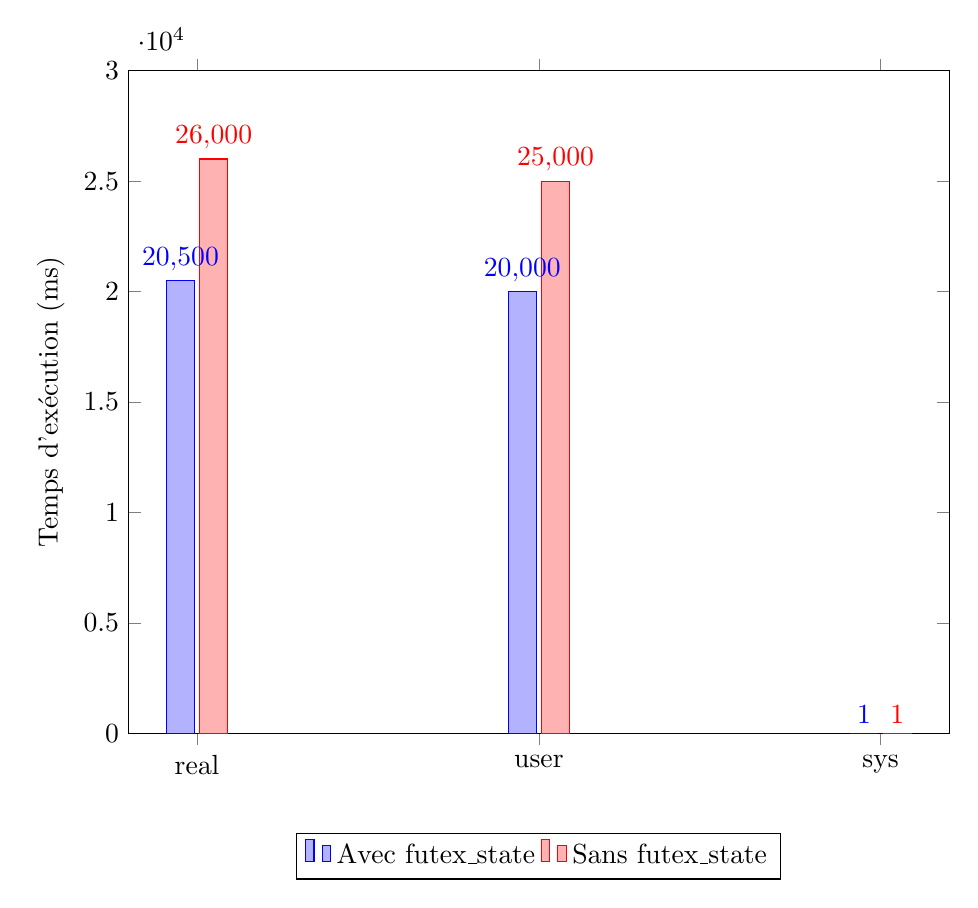
\begin{tikzpicture}
	\begin{axis}[
	ybar,
	ymin=0, ymax=30000,
	legend style={at={(0.5,-0.15)},
		anchor=north,legend columns=-1},
	ylabel={Temps d'exécution (ms)},
	symbolic x coords={real,user,sys},
	xtick=data,
	nodes near coords,
	nodes near coords align={vertical},
	width=12cm,height=10cm,
	]
	\addplot coordinates {(real,20500) (user,20000) (sys,1)};
	\addplot coordinates {(real,26000) (user,25000) (sys,1)};
	\legend{Avec futex\_state, Sans futex\_state}
	\end{axis}
	\end{tikzpicture}
	\caption{Overhead}
	\label{fig:overhead}
\end{figure}



\noindent \textbf{Résultat:}
Temps d'exécution \textbf{sans} notre implémentation des futex state:
\begin{lstlisting}
real	0m43.359s
user	0m43.326s
sys	0m0.011s
\end{lstlisting}
Le thread parent ne fini pas avant les threads parallèles.

\noindent Temps d'exécution \textbf{avec} notre implémentation des futex state:
\begin{lstlisting}
real	0m4.406s
user	0m4.396s
sys	0m0.003s
\end{lstlisting}
Le thread parent fini bien avant les threads parallèles.

Par manque de temps nous n'avons pas pu évaluer notre implémentation sur des scénarios plus complexes,
notamment en jouant avec le multicœur. 